\section{Warehouse-Scale Computers}

The rise of server-side computing and the widespread adoption of internet services have given rise to a new class of computing systems known as Warehouse-Scale Computers (WSCs). 
In WSC, the program:
\begin{itemize}
    \item Operates as an internet service.
    \item Can comprise tens or more individual programs.
    \item These programs interact to deliver complex end-user services like email, search, maps, or Machine Learning (ML).
\end{itemize}
Data centers are facilities where numerous servers and communication units are housed together due to their shared environmental needs, physical security requirements, and streamlined maintenance. 
Traditional data centers typically accommodate a considerable number of relatively small or medium-sized applications, each operating on dedicated hardware infrastructure isolated and safeguarded against other systems within the same facility. 
These applications typically do not communicate with one another, and data centers often host hardware and software for multiple organizational units or even different companies.

In contrast, WSCs are owned by a single organization, employ a relatively uniform hardware and system software platform, and share a unified systems management layer.
\begin{figure}[H]
    \centering
    \begin{subfigure}{0.49\textwidth}
        \centering
        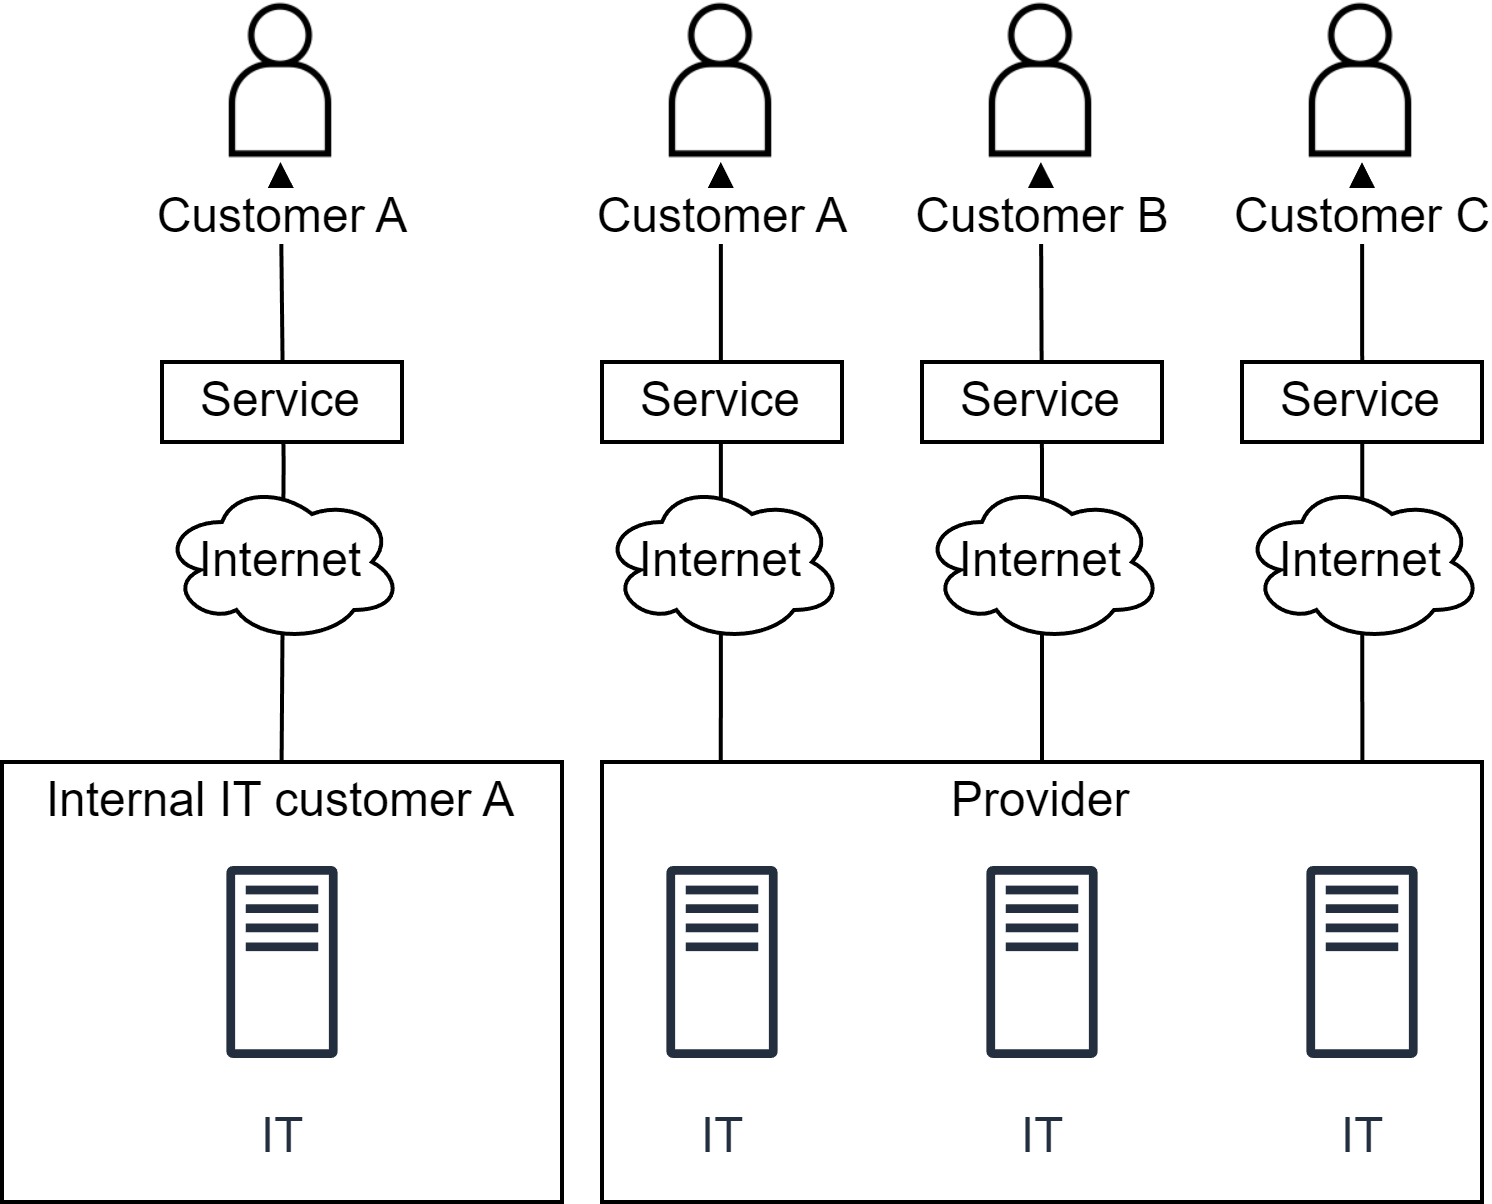
\includegraphics[width=0.75\linewidth]{images/datacenter.png} 
        \caption{Data center}
    \end{subfigure}
    \begin{subfigure}{0.49\textwidth}
        \centering
        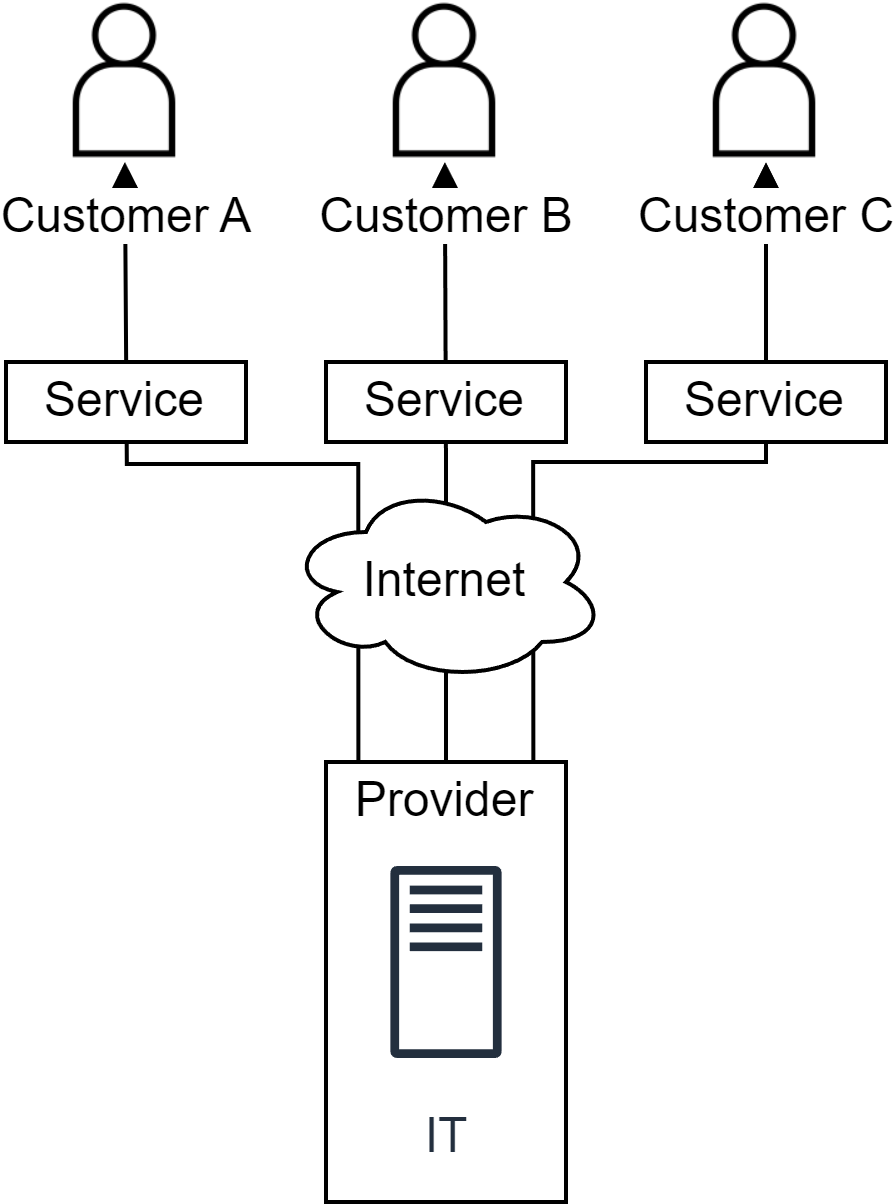
\includegraphics[width=0.45\linewidth]{images/warehouse.png}
        \caption{Data warehouse}
    \end{subfigure}
    \caption{Structures of data centers and data warehouses}
\end{figure}
WSCs operate a reduced quantity of highly expansive applications, often internet services. 
Their shared resource management infrastructure affords considerable deployment flexibility. 
Designers are driven by the imperatives of homogeneity, single-organization control, and cost efficiency, prompting them to adopt innovative approaches in crafting WSCs.

Originally conceived for online data-intensive web workloads, WSCs have expanded their capabilities to drive public cloud computing systems, such as those operated by Amazon, Google, and Microsoft. 
These public clouds accommodate numerous small applications, resembling a traditional data center setup. 
However, all these applications leverage virtual machines or containers and access shared, large-scale services for functionalities like block or database storage and load balancing, aligning seamlessly with the WSC model.

The software operating on these systems is designed to run on clusters comprising hundreds to thousands of individual servers, far surpassing the scale of a single machine or a single rack. 
The machine itself constitutes this extensive cluster or aggregation of servers, necessitating its consideration as a single computing unit.

Services offered by WSCs need to ensure high availability, usually targeting a minimum uptime of 99.99\%, equating to one hour of downtime per year. 
Maintaining flawless operation is challenging when managing a vast array of hardware and system software components. 
Therefore, WSC workloads must be crafted to gracefully handle numerous component faults, minimizing or eliminating any adverse effects on service performance and availability.

\subsection{Architecture}
While the hardware implementation of WSCs may vary considerably, the architectural organization of these systems remains relatively consistent.
\begin{figure}[H]
    \centering
    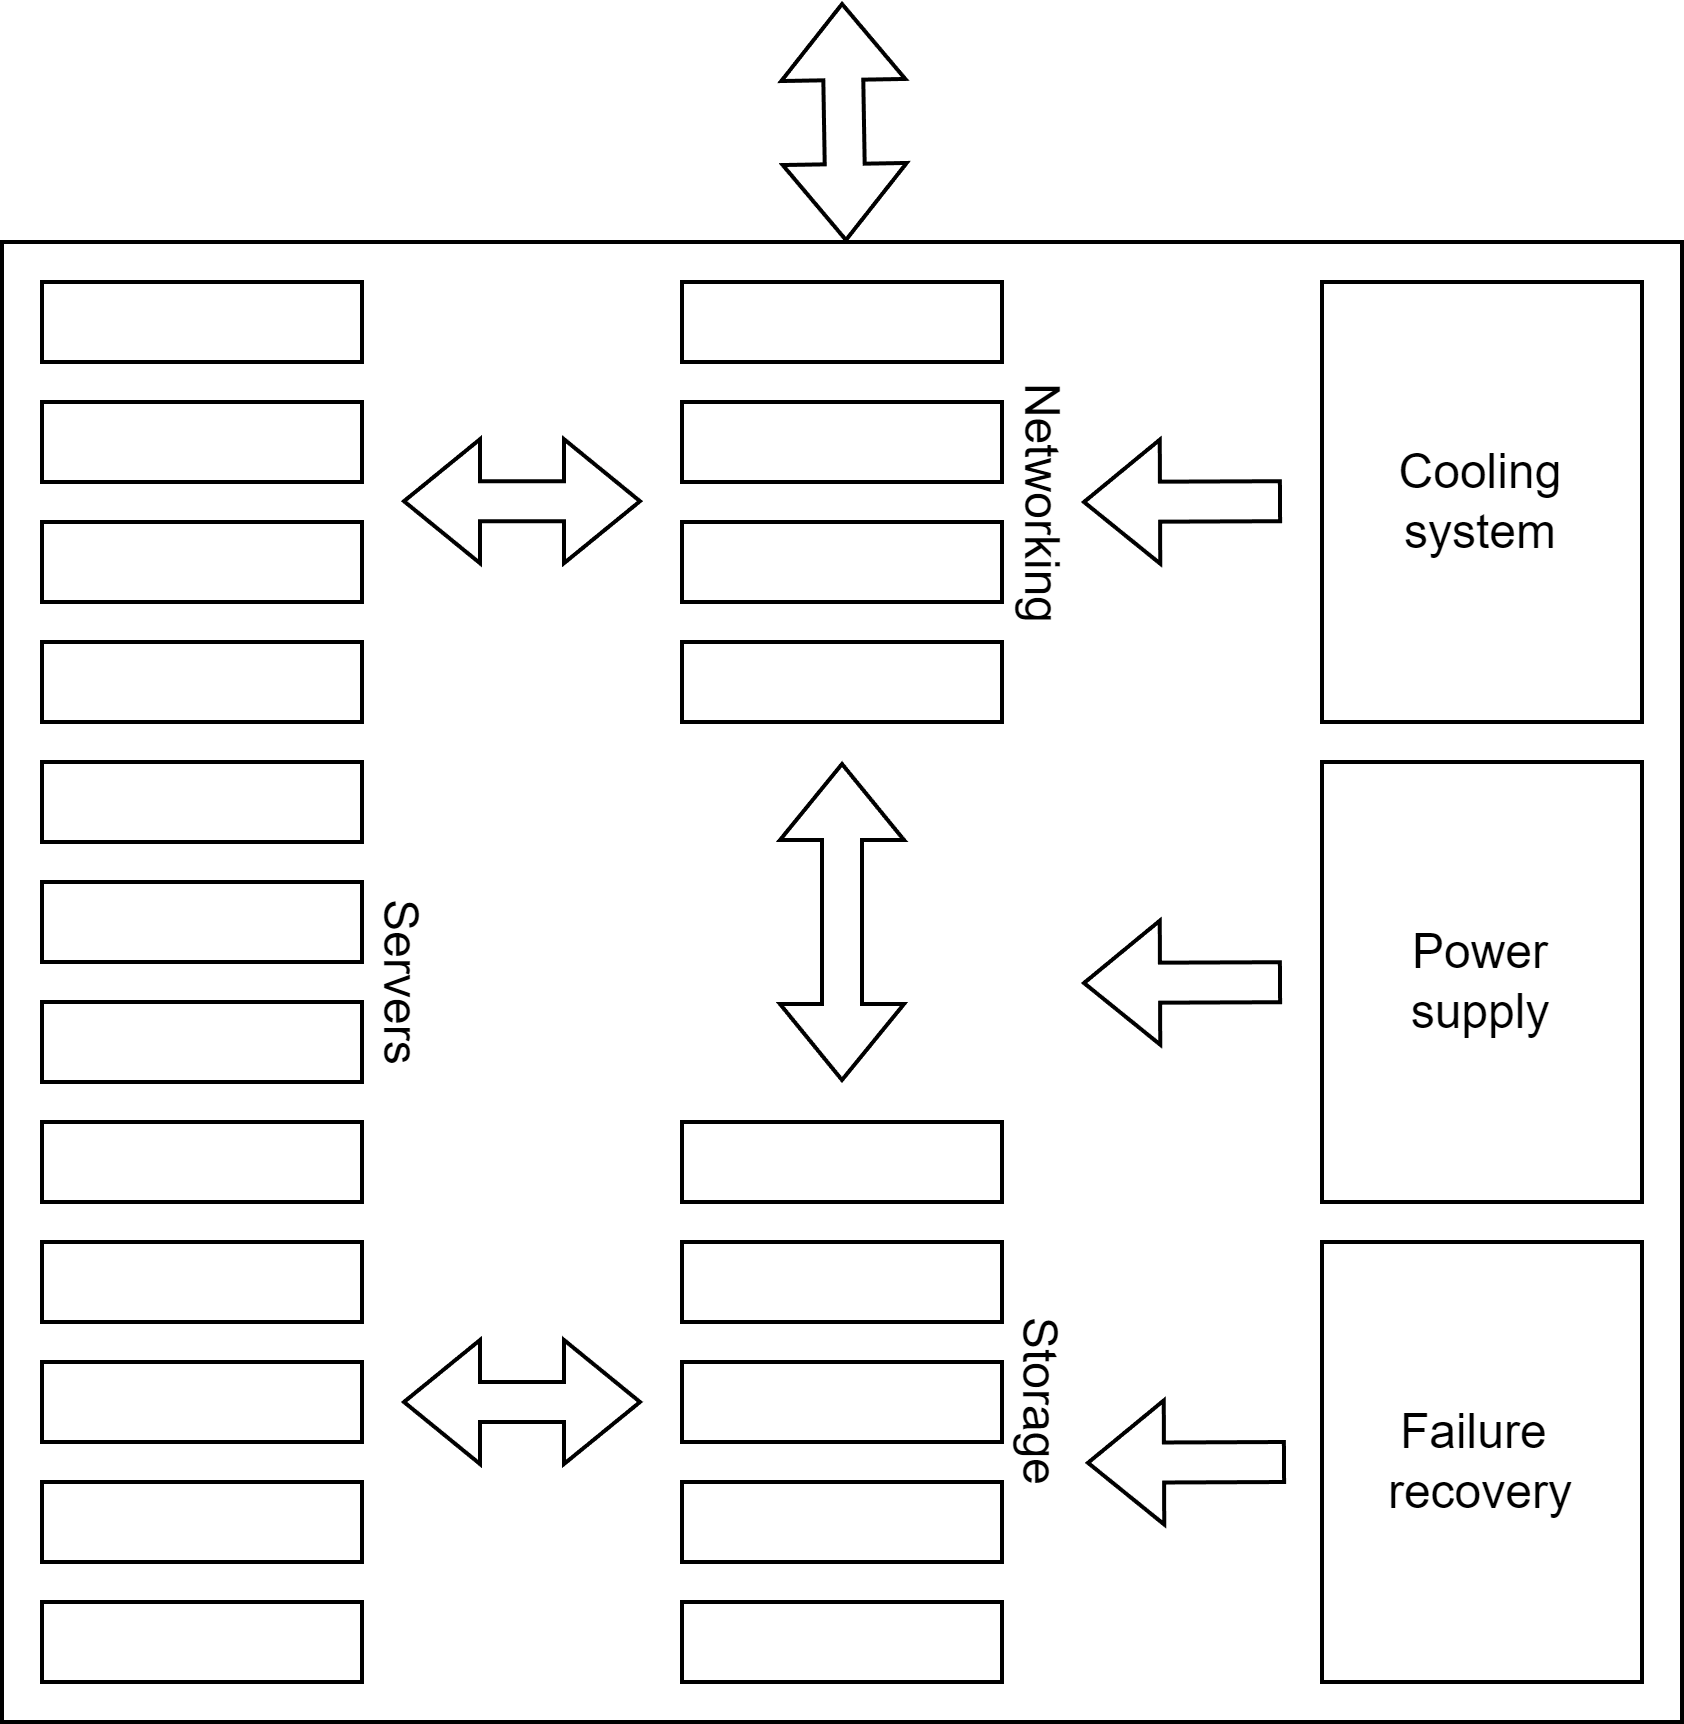
\includegraphics[width=0.5\linewidth]{images/infr.png}
    \caption{Architecture of WSC}
\end{figure}

\paragraph*{Servers}
Servers resemble standard PCs but are designed with form factors that enable them to fit into racks, such as racks, blade enclosure format, or tower configurations. 
They can vary in terms of the number and type of CPUs, available RAM, locally attached disks (HDD, SSD, or none), as well as the inclusion of other specialized devices like GPUs and coprocessors.

\paragraph*{Storage}
Disks and Flash SSDs serve as the fundamental components of contemporary WSC storage systems. T
These devices are integrated into the data-center network and overseen by advanced distributed systems. 

\paragraph*{Networking}
Communication equipment facilitates network interconnections among devices within the system. 
These include hubs, routers, DNS or DHCP servers, load balancers, switches, firewalls, and various other types of devices.